\section{Implemented object detection algorithm and Evolution of YOLO model} \vspace{-2em}
\subsection{YOLO}
YOLO (You Only Look Once) is an object detection system used for real-time object detection. It was introduced in 2016 by Joseph Redmon, Santosh Divvala, Ross Girshick, and Ali Farhadi. YOLO is known for its high speed and accuracy. The system is designed to classify and detect multiple objects in an image using a single forward pass of the neural network.
Traditional object detection systems use a sliding window approach where they apply a classifier at each location and scale of the image. This process is computationally expensive and time-consuming. On the other hand, YOLO divides the input image into a grid of cells and each cell is responsible for detecting an object. This approach reduces the number of bounding boxes that need to be processed and allows for real-time detection, this make it suitable for a wide range of applications such as self-driving cars, surveillance systems, and robotics. Additionally, YOLO can detect objects at different scales and aspect ratios, making it robust to variations in object size and orientation. \cite{terven2023comprehensive} \cite{redmon2016you} \href{https://deci.ai/blog/history-yolo-object-detection-models-from-yolov1-yolov8/}{\textcolor{blue}{Ref 1}}\\
2. \href{https://deci.ai/blog/yolov8-vs-yolo-nas-showdown-exploring-advanced-object-detection/}{\textcolor{blue}{[Ref]}}
3. \href{https://arxiv.org/pdf/2304.00501.pdf}{\textcolor{blue}{Ref: 3}}

\subsection{The Evolution of YOLO}
\begin{figure}[H]
    \centering
    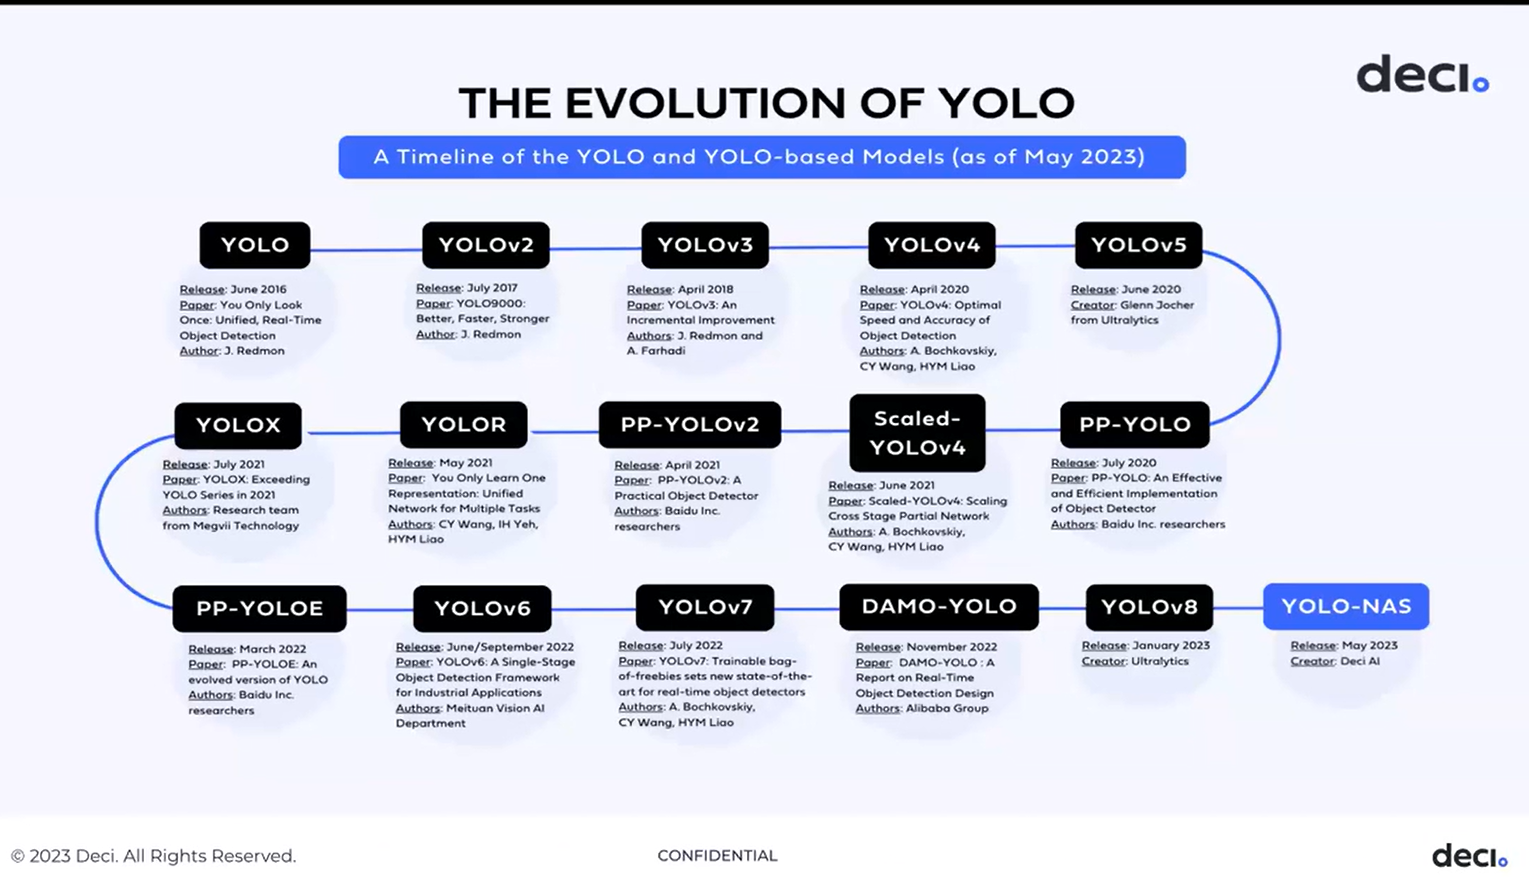
\includegraphics[width=\textwidth]{evolution_of_YOLO.PNG}
    \caption{The evolution  of yolo [Source: \href{https://deci.ai/resources/webinar-open-source-llms-vs-apis/}{\textcolor{blue}{Deci. ai webinar}}]}
    \label{fig:YOLO-Evolution}
\end{figure}
\begin{enumerate}
    \item \textbf{YOLO: } YOLO introduced in 2016 for real-time object detection.
    Achieved a groundbreaking mAP of 63.4\% on PASCAL VOC2007 dataset.
    YOLO's efficiency in one network pass.
    Localization error limitations due to object count, aspect ratios, and down-sampling. \cite{redmon2016you}\\
    \item \textbf{YOLOv2 Improvements: } YOLOv2 introduced in 2017 with 9000+ categories.
    Improved with batch normalization, high-resolution classifier, and anchor boxes.
    Joint training for classification and detection.\cite{sang2018improved}\\
    \item \textbf{YOLOv3 Advancements: } YOLOv3 (2018) achieved 60.6\% mAP on MS COCO, 2x faster than previous versions.
    Introduced logistic regression for objectness scores and anchor box priors. \cite{redmon2018yolov3}\\
    \item \textbf{YOLOv4 Global Impact: } YOLOv4 (2020) maintained YOLO's philosophy with bag-of-freebies and bag-of-specials. Enhanced accuracy with image adjustments like mosaic augmentation and DropBlock. \cite{gai2023detection}
    \item \textbf{YOLOv5 Speed and Efficiency: } YOLOv5 (2020) by Ultralytics in PyTorch achieved 50.7\% AP with user-friendly features. \cite{wu2021real}\\
    \item \textbf{YOLOX Anchor-Free Innovation: } YOLOX (July 2021) exceeded previous YOLO versions, anchor-free with center sampling. Employed MixUP, Mosaic augmentations for improved accuracy. \cite{ge2021yolox}\\
    \item \textbf{YOLOR Multi-Task Learning: } YOLOR (May 2021) focused on a unified network for multiple tasks.
    Applied multi-task learning for classification, detection, and pose estimation.\\

    \item \textbf{PP-YOLOv2: }  Upgrades include ResNet101, PAN, Mish Activation, increased input size, and modifications to IoU-aware branch. \cite{huang2021pp}\\
    \item \textbf{Scaled-YOLOv4 Flexibility: } Scaled-YOLOv4 (CVPR 2021) introduced scaling-up and scaling-down techniques. YOLOv4-tiny for low-end GPUs, YOLOv4-large for cloud GPUs. \cite{wang2021scaled}\\ 
    \item \textbf{PP-YOLO: } A YOLOv3-based model by Baidu, leveraging PaddlePaddle, introducing ten tricks for accuracy without sacrificing speed.\cite{long2020pp}\\
    \item \textbf{PP-YOLOE: } Evolved from PP-YOLOv2 with anchor-free architecture, new backbone, TAL, ET-head, and VFL/DFL. \cite{xu2022pp}\\
    \item \textbf{YOLOv6 Industrial Framework: } 
    YOLOv6 (September 2022) for industrial applications with anchor-free detection.
    YOLOv6-L achieved 52.5\% AP and 70\% AP50 at 50 FPS. \cite{li2022yolov6}, \cite{terven2023comprehensive}
    \item \textbf{YOLOv7 Speed and Accuracy: } YOLOv7 (July 2022) surpassed others in speed and accuracy.
    E-ELAN, model scaling, and "bag-of-freebies" approach for efficiency. \cite{wang2023yolov7}, \cite{terven2023comprehensive}\\
    \item \textbf{DAMO-YOLO Real-Time Improvements: } DAMO-YOLO (November 2022) by Alibaba for real-time object detection. 
    Introduced MAE-NAS, Efficient-RepGFPN, ZeroHead, and knowledge distillation. \cite{xu2022damo}\\
    \item \textbf{YOLOv8 :}
    YOLOv8 (January 2023) by Ultralytics with anchor-free prediction and faster NMS. Mosaic augmentation during training for improved accuracy.
    YOLOv8 offers five scaled versions: YOLOv8n (nano), YOLOv8s (small), YOLOv8m (medium), YOLOv8l (large), and YOLOv8x (extra\-large). YOLOv8x outperformed YOLOv5 on the MS COCO dataset with an impressive 53.9\% AP at 640 pixels and fast speed.\cite{yolov8}, \cite{terven2023comprehensive}
\end{enumerate}
\href{https://www.mdpi.com/2504-4990/5/4/83}{\textcolor{blue}{Source}}
\subsection{YOLO-NAS}
YOLO-NAS is a cutting-edge object detection model created using Deci's Neural Architecture Search technology, AutoNAC™. It offers unmatched real-time object detection capabilities and production-ready performance, surpassing other models such as YOLOv5, YOLOv6, YOLOv7, and YOLOv8.

The YOLO-NAS model undergoes a multi-phase training process, which involves pre-training on Objects365, COCO Pseudo-Labeled data, Knowledge Distillation (KD), and Distribution Focal Loss (DFL).

During the pre-training phase, the model is trained on Objects365, a comprehensive dataset that consists of 2 million images and 365 categories. Depending on the model variant, this process can take 25-40 epochs, as each epoch requires 50-80 minutes on 8 NVIDIA RTX GPUs. 

In addition, the COCO dataset provides an extra 123k unlabeled images, which are used to generate pseudo-labeled data. An accurate model is trained on COCO to label these images, which are then used to train our model with the original 118k train images.

Moreover, the YOLO-NAS architecture uses Knowledge Distillation (KD) and Distribution Focal Loss (DFL) techniques to enhance its training process.
YOLO-NAS training procedure is comprehensive and leverages multiple datasets, labelled and unlabelled, and supervised and unsupervised training procedures. \cite{YOLO-NAS}, \cite{terven2023comprehensive}
\begin{figure}[H]
    \centering
    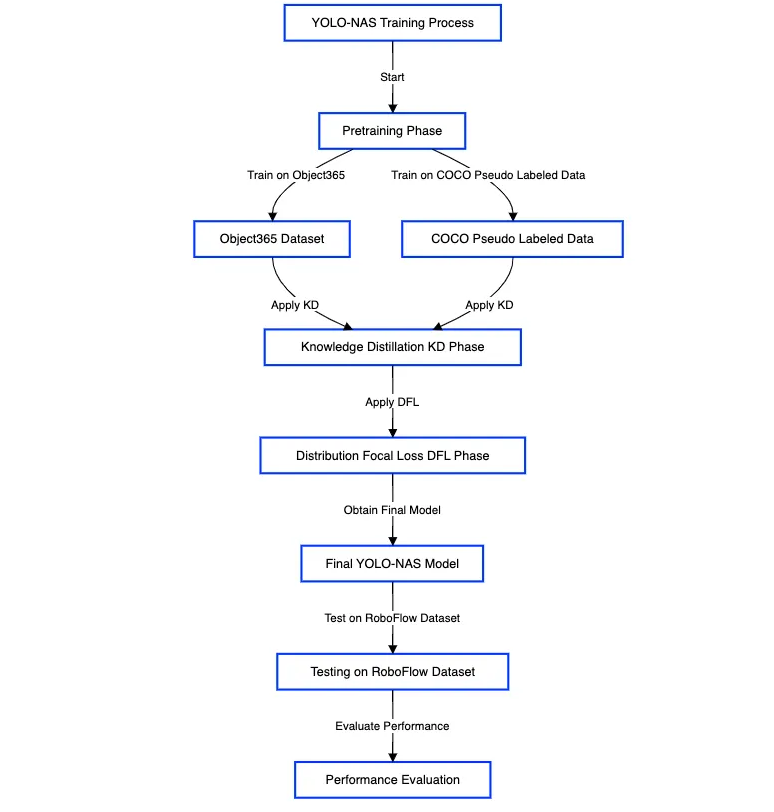
\includegraphics[width=0.8\textwidth]{YOLO-NAS-Training.PNG}
    \caption{An overview of the YOLO-NAS training process \cite{richmond_yolo-nas} \href{https://richmondalake.medium.com/yolo-nas-uncovered-essential-insights-and-implementation-techniques-for-machine-learning-engineers-87ee266b37f6}{\textcolor{blue}{Source}}}
    \label{fig:enter-label}
\end{figure}
\href{https://deci.ai/blog/yolo-nas-object-detection-foundation-model/}{\textcolor{blue}{Source-1}}
\href{https://deci.ai/model-zoo/yolo-nas/}{\textcolor{blue}{Source-2}}  



\subsubsection{Architectural Features of YOLO-NAS} \vspace{0mm}It is considered one of the most efficient object detection algorithms due to its unique architecture, which is designed to minimize the computational cost of the algorithm while maintaining high accuracy. \cite{yolo-nas-vs-yolov8}[\href{https://deci.ai/blog/yolov8-vs-yolo-nas-showdown-exploring-advanced-object-detection/#:~:text=Quantization%20Aware%20Blocks%20and%20Selective%20Quantization&text=This%20architecture%20utilizes%20Quantization%2DSpecific,parameterization%20with%208%2Dbit%20quantization.}{\textcolor{blue}{Source: 1}}]   
\begin{enumerate}
    \item \textbf{Quantization Aware Blocks and Selective Quantization: } 
        \begin{itemize}
            \item \textbf{Hybrid Quantization Method: } YOLO-NAS employs a hybrid quantization strategy, integrating Quantization-Specific Parameters (QSP) and Quantization-Centric Initialization (QCI) blocks. These leverage re-parameterization and 8-bit quantization, inspired by Chu et al.'s methodology.
            \item  \textbf{Selective Quantization:} The model strategically quantizes specific parts rather than uniformly affecting all layers. This selective quantization balances accuracy and latency, addressing information loss, a common issue in standard quantization techniques.
                \item \textbf{Layer Selection Algorithm:} YOLO-NAS utilizes a sophisticated layer selection algorithm to decide which layers to quantize. It evaluates the impact of each layer on accuracy and latency, carefully considering the implications of toggling between 8-bit and 16-bit quantization.
                \item \textbf{Performance in Limited Resources:} Uniquely designed for environments with limited resources, YOLO-NAS ensures superior performance. Its optimized approach to quantization preserves accuracy while being efficient, striking a crucial balance for advanced object detection tasks.
        \end{itemize}
    \item \textbf{Detection Head: } A standout feature of YOLO-NAS is its detection head design, which predicts a distribution probability for size regression. This approach is particularly useful in scenarios where the object sizes vary significantly. By predicting a range of possible sizes rather than a single fixed size, YOLO-NAS enhances its accuracy in detecting objects of varying scales. This probabilistic approach to size regression also makes YOLO-NAS suitable for knowledge distillation. It allows for a more nuanced transfer of knowledge from a complex, high-capacity teacher model to a simpler, more efficient student model, further enhancing the practicality of YOLO-NAS in diverse applications.
    \item \textbf{Neck: } The YOLO-NAS network has a highly advanced pyramid-attention neck that combines both top-down and bottom-up information flows. 
    \begin{figure}[H]
        \centering
        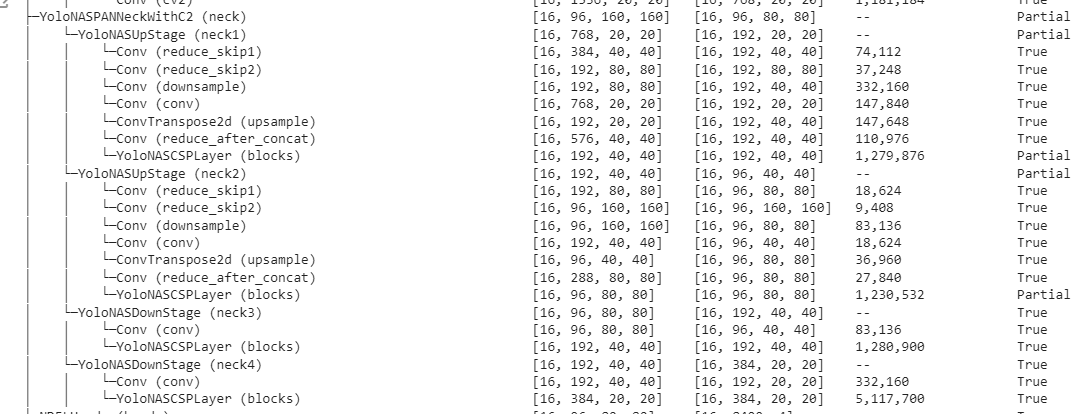
\includegraphics[width=\textwidth]{yolo-nas_neck.PNG}
        \caption{Neck Design}
        \label{fig:Neck}
    \end{figure}
    This design element assists the network in effectively capturing and utilizing multi-scale information. In this pyramid-attention structure, the top-down pathway captures high-level semantic information, while the bottom-up pathway focuses on smaller details. The attention mechanism in this pyramid structure ensures that the network focuses on the most relevant features at different scales, which improves its ability to detect objects with varying sizes and complexities. 
    \item \textbf{Backbone: } 
The backbone of YOLO-NAS, a pivotal component in its architecture, is a product of an advanced Network Architecture Search (NAS) process, specifically utilizing Deci’s proprietary NAS technology, AutoNAC. This innovative approach enables the tailoring of the network structure to meet the specific demands of object detection tasks with unparalleled precision.
\begin{itemize}
    \item \textbf{quantization-aware RepVGG: } During the NAS process, they have incorporated quantization-aware RepVGG blocks into the model architecture, ensuring that our model architecture would be compatible with Post-Training Quantization (PTQ).\\
    \item \textbf{Spatial Pyramid Pooling (SPP): } YOLO-NAS backbone has Spatial Pyramid Pooling (SPP)  at the end to capture global context, it is a pooling layer that removes the fixed-size constraint of the network, i.e. a CNN does not require a fixed-size input image. Placing SPP at the end of the YOLO-NAS backbone allows the model to capture global context information, which is crucial for understanding the overall context of the scene. This can be beneficial for detecting objects that may span a larger region in the image.
\end{itemize}

\href{https://deci.ai/blog/yolo-nas-object-detection-foundation-model/}{Source}

\begin{figure}[H]
    \centering
    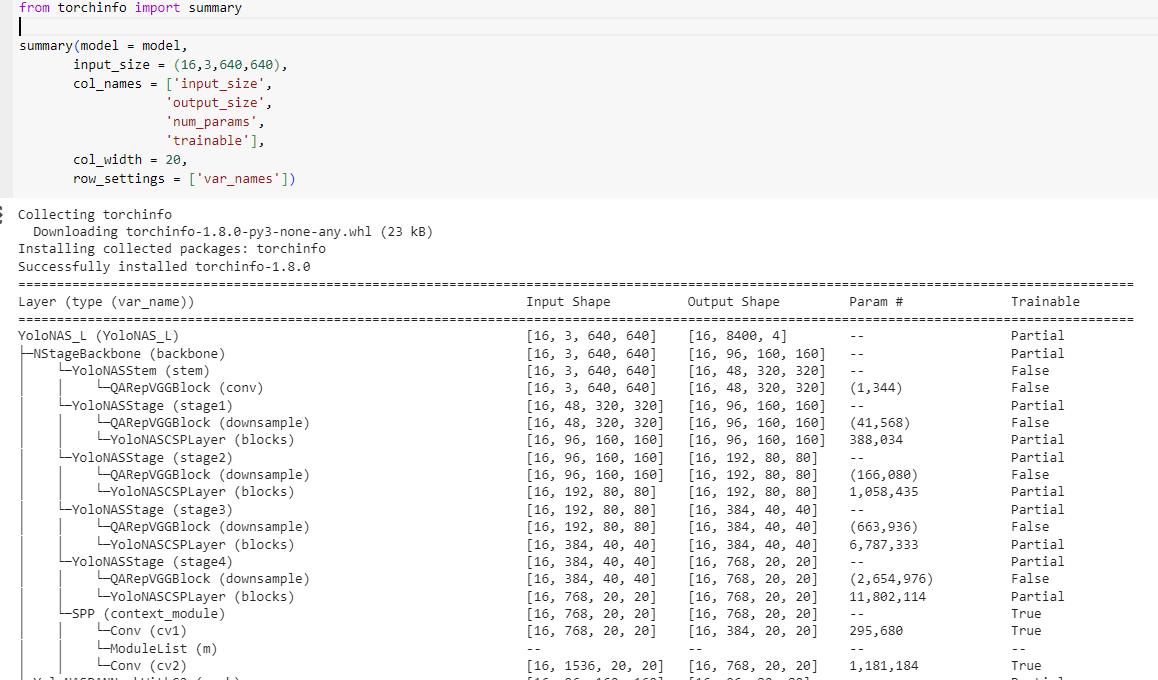
\includegraphics[width=\textwidth]{Yolo-BackBone.PNG}
    \caption{Backbone Structure}
    \label{fig:BackBone}
\end{figure}

AutoNAC, as a part of the NAS process, plays a critical role in determining the optimal sizes and structures of various stages within the YOLO-NAS backbone. This includes meticulously configuring the block type, the number of blocks, and the number of channels in each stage. By doing so, AutoNAC ensures that each aspect of the backbone is precisely optimized for its function.

The NAS-generated backbone, therefore, is not just a result of automated design but also of intelligent decision-making that considers a multitude of factors. This includes computational efficiency, accuracy, and speed, ensuring that the backbone contributes effectively to the overall robustness and adaptability of YOLO-NAS.

These advancements culminate in a superior architecture with unprecedented object detection capabilities and outstanding performance over its predecessors.
\end{enumerate} 

\subsubsection{Automated Neural Architecture Construction (AutoNAC) engine}
Deci-AI utilizes an optimization engine called AutoNAC, which was developed by Deci. This engine applies Neural Architecture Search (NAS) to enhance the architecture of a deep learning model. The main goal is to improve the performance of the model when it is executed on specific hardware while maintaining or even improving its accuracy. The AutoNAC engine is hardware aware, data-aware and considers all the components in the inference stack, including compilers and quantization. \\
AutoNAC is essentially a NAS engine takes three components as inputs. \cite{yolo-nas-webinar}
\begin{itemize}
    \item \textbf{Task: } Firstly, we need to decide which model to build, such as an object detection model.\\
    \item \textbf{Data characteristics: } Deci Group requires the NAS Engine to be data-aware or capable of understanding the characteristics of the data so that it can create a model that is well-suited for the task at hand. For instance, if the objective is to detect small objects, the model would likely be different from that required for detecting large objects, as the receptive fields would differ. \\
    \item \textbf{Inference environment and Hardware: } When it comes to computer vision on edge, the priority is to achieve real-time performance or improve some level of latency or throughput while being hardware-aware, compilation-aware, and quantization-aware. To achieve this, we need to consider factors such as model size, latency, and throughput. Decis Group's goal is to optimize these factors as part of the Neural Architecture Search (NAS) process. Manually finding the optimal architecture for object detection models can be a laborious and inefficient process. To address this issue, Deci utilized AutoNAC, a tool that uses neural design space incorporating state-of-the-art (SOTA) architectural design principles and Deci's novel neural elements, to discover novel object detection models. These models were optimized to minimize inference latency computed over NVIDIA's T4 cloud GPU, which is a widely used computing device. We achieve this by feeding all three inputs into the AutoNAC engine, which generates a new architecture.
\end{itemize}
 
\begin{figure}[H]
    \centering
    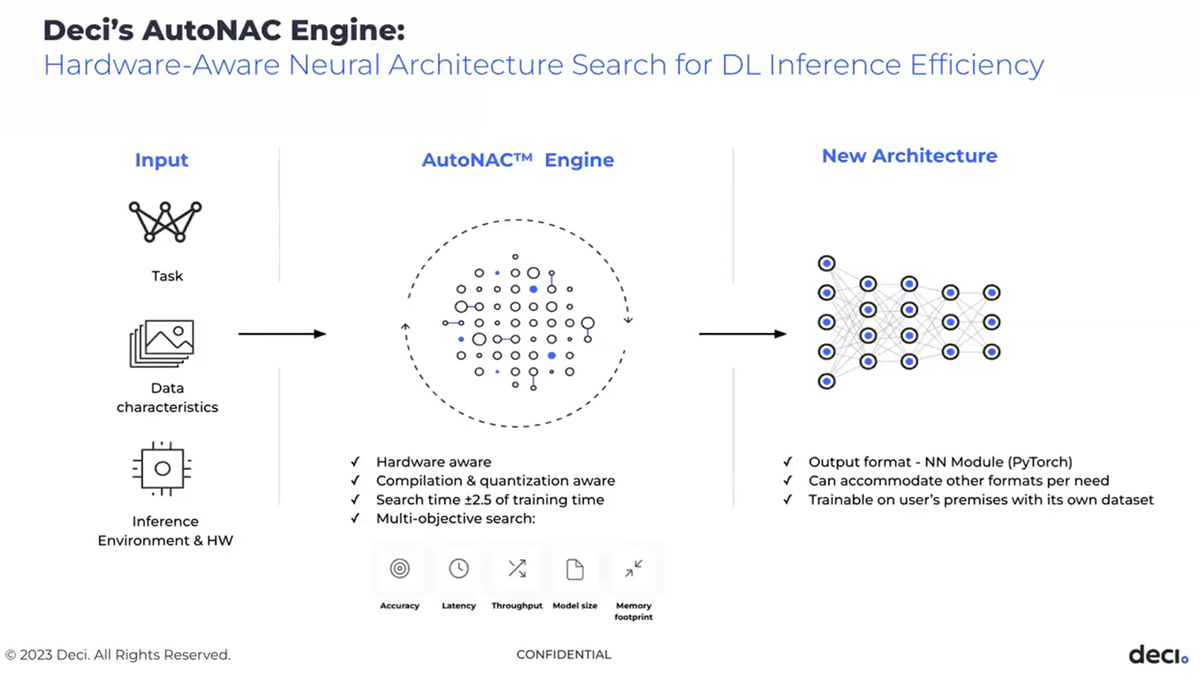
\includegraphics[width=\textwidth]{autoNAC_Engine.PNG}
    \caption{Deci's AutoNAC Engine; \\
    Hardware-Aware Neural Architecture Search for DL Inference Efficiency}
    \label{fig:AutoNAC Engine}
\end{figure}

\subsubsection{Under the hood View of Auto-NAC}
NAS algorithms can systematically explore the vast search space of potential architectures, effectively identifying novel and optimized configurations that might be overlooked by human intuition. By automating the process, these algorithms can efficiently evaluate and compare a vast number of candidate architectures with an unfathomable search space of $10^{14}$ possible architectures, ultimately converging on a solution that optimally balances accuracy, speed, and complexity, and the NAS engine comes into place when we have data already and want to build a model.
it takes all three above-mentioned inputs, and the search space is automatically created under the hood taking into account all the possibilities of Neural Architecture as an input. For Example, opti mal sizes, block types, number of blocks, and channel counts in every stage. \cite{yolo-nas-webinar}  \href{https://deci.ai/blog/sota-dnns-overview/}{\textcolor{blue}{Source}}  
\begin{figure}[H]
    \centering
    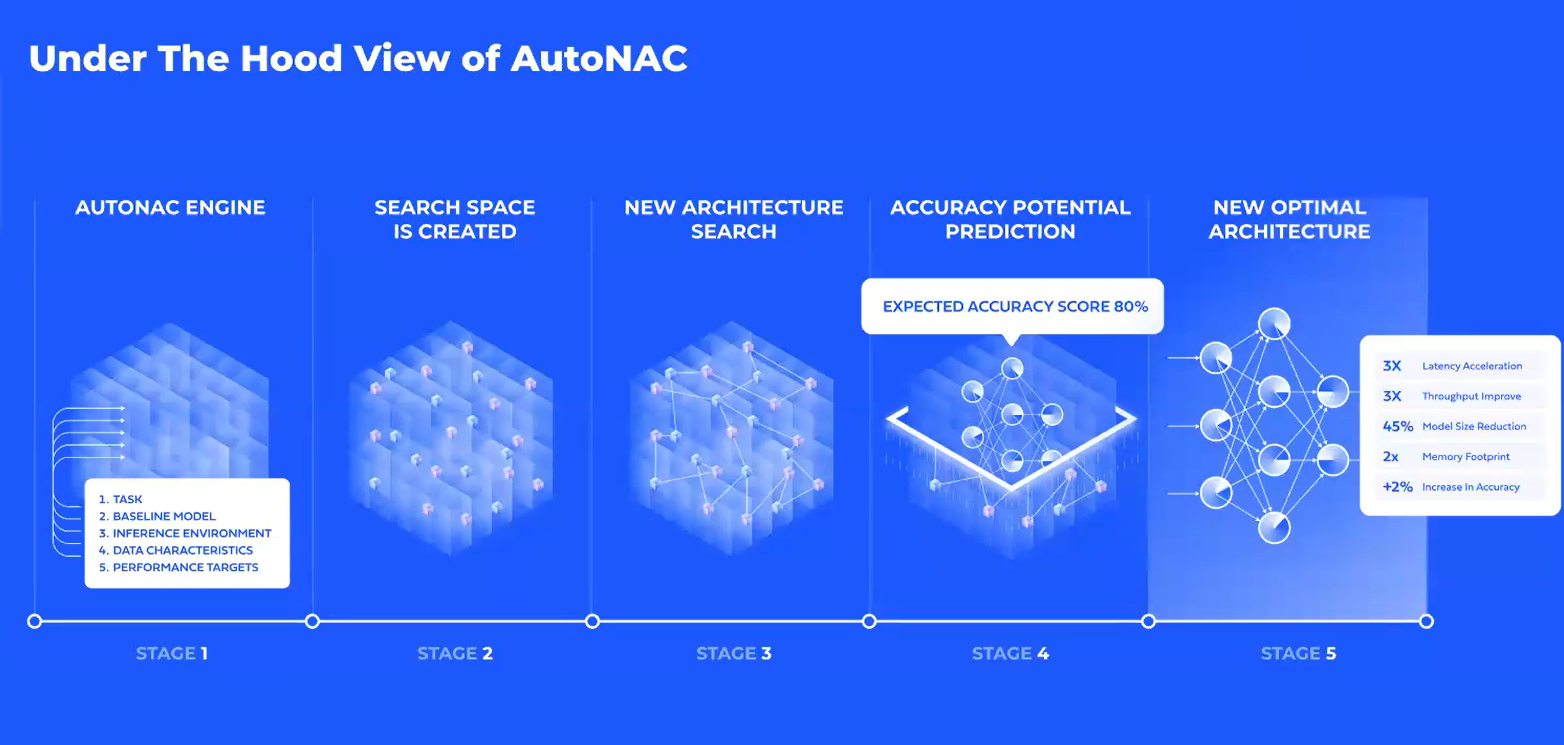
\includegraphics[width=\textwidth]{AUTONACENGINE_Underthe hood.PNG}
    \caption{AutoNAC Engine Search Space}
    \label{fig:autonac_under_the_hood}
\end{figure}
Finally, AutoNAC Engine explores and maps the efficiency frontier, searching for an architecture that best balances latency vs. throughput. Deci Group samples three points of this frontier to create the YOLO-NASS, YOLO-NASM, and YOLO-NASL architectures.
\subsubsection{How to find the best architecture out of the search space}
while the search space has trillions of candidate architectures, the task of identifying the optimal architecture becomes increasingly challenging. Within the realm of Deci, the selection of the most suitable candidate from the numerous models within the extensive search space is guided by two distinct evaluation criteria. \cite{yolo-nas-webinar}
\begin{enumerate}
    \item \textbf{Bench Marking: } Understanding how the model will behave on the expected hardware or using the techniques of Latency Vs. throughput for the candidate architecture. \\
    \item \textbf{Accuracy Potential Predictions: } The fundamental selection methodology of best candidate out of the search space involves the provision of an AI model, designated to assess the accuracy or potential accuracy of neural network models. Leveraging principles from neural architecture search, YOLO-NAS systematically navigates the expansive design space of possible neural network configurations, employing optimization algorithms to identify architectures anticipated to yield high accuracy on the specified object detection task.
\end{enumerate}
 \begin{figure}[H]
     \centering
     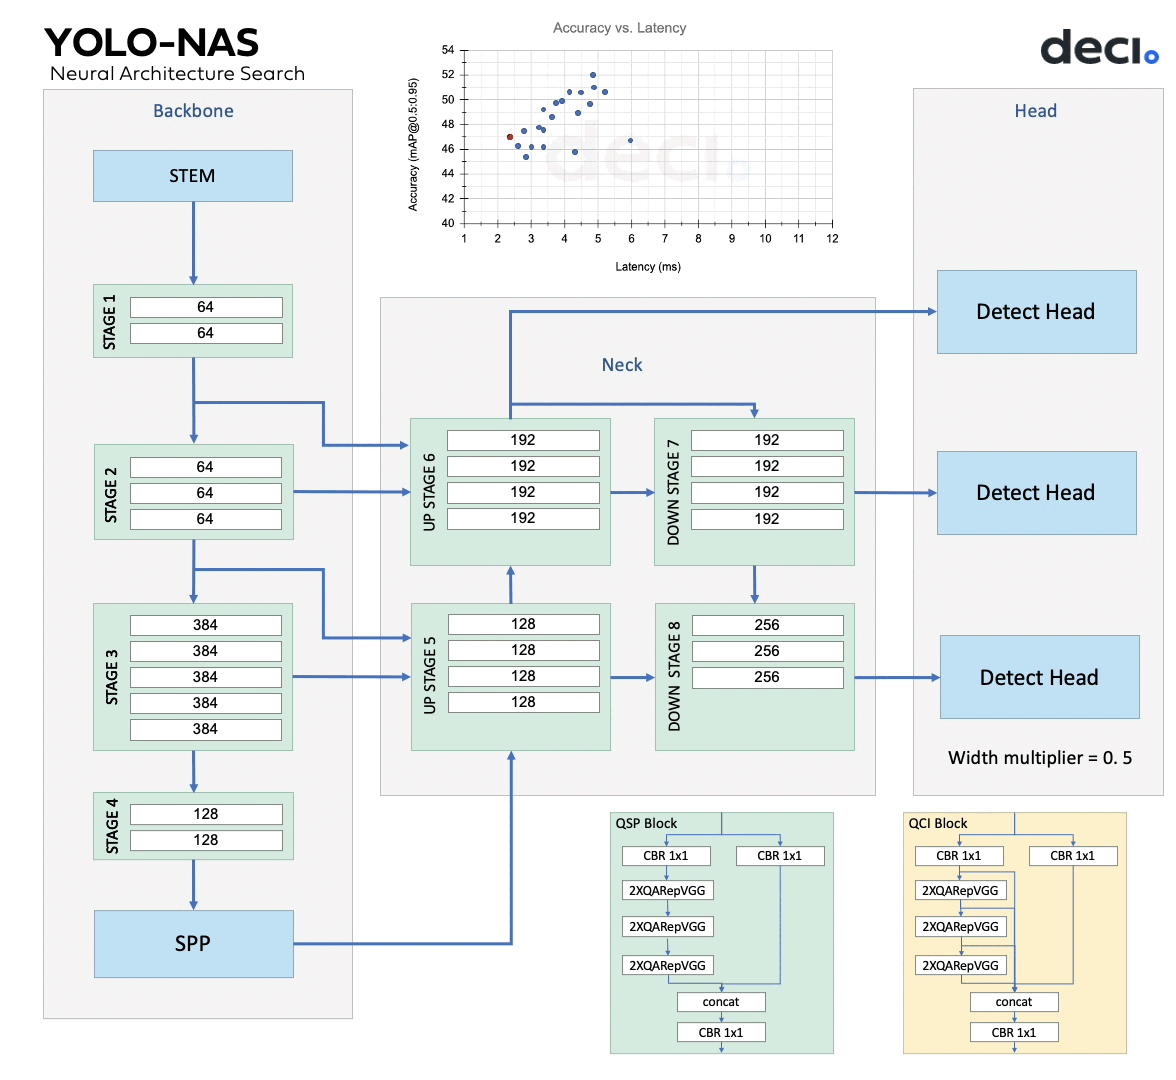
\includegraphics[width=\textwidth]{Yolo_nas.png}
     \caption{\textbf{YOLO-NAS Architecture. The architecture is found automatically via a Neural Architecture Search(NAS) system called AutoNAC to balance latency vs. throughput. They generated three architecture called YOLO-NASS(small), YOLO-NASM(medium), and YOLO-NASL(large), varying the depth and the position of the QSP and QCI blocks \cite{YOLO-NAS}}}
     \label{fig:YOLO-NAS Architecture.}
\end{figure}


\subsubsection{Fine-tuning of the selected model On custom data set}
Fine-tuning is the process of making small adjustments to achieve the desired output or performance. In deep learning, it involves the use of weights of a trained neural network to program another deep learning algorithm from the same domain. The weights connect each neuron in one layer to every neuron in the next layer in the neural network. Fine tuning is used to speed up the training and/or overcome a small dataset as it already contains vital information from a pre-existing deep learning algorithm. The YOLO-NAS architecture and pre-trained weights define a new frontier in low-latency inference and an excellent starting point for fine-tuning downstream tasks. Strong pre-trained weights often lead to higher model accuracy on new datasets when fine-tuning. YOLO-NAS was trained on the RoboFlow100 dataset (RF100), a collection of 100 datasets from diverse domains, to demonstrate its ability to handle complex object detection tasks. The RF100 dataset is a benchmark for existing YOLO models, enabling us to compare YOLO-NAS’s performance against them and showcase its advantages.\cite{YOLO-NAS}
\begin{figure}[H]
    \centering
    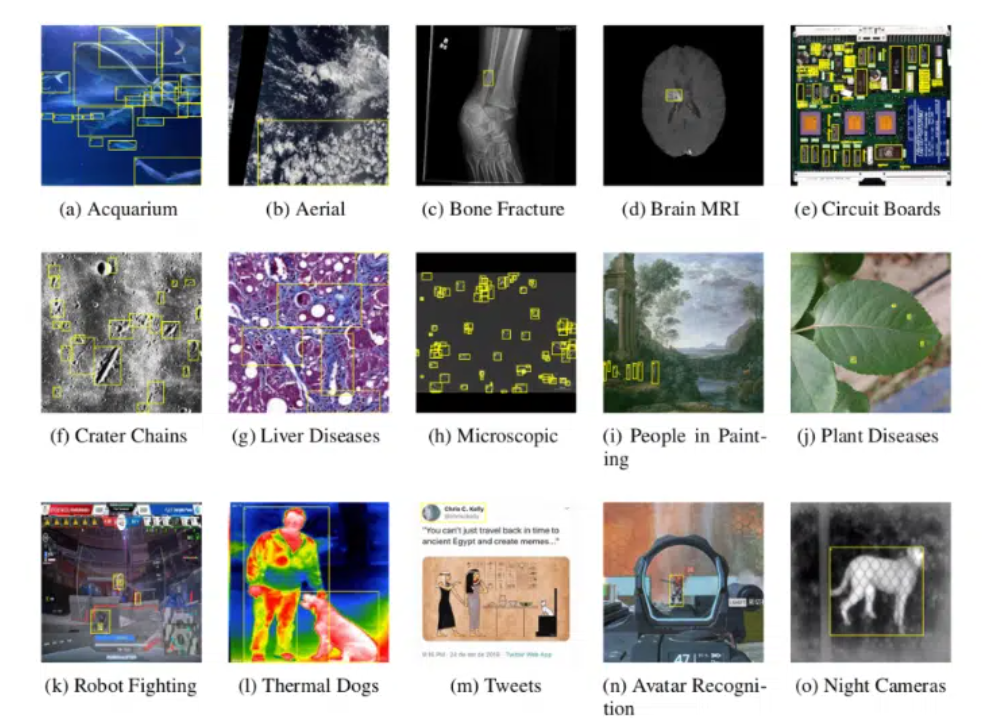
\includegraphics[width=0.8\textwidth]{YOLO-NAS_RF100_benchmark.PNG}
    \caption{Examples of annotated images in the RF100 benchmark}
    \label{fig:YOLO-NAS_RF100_benchmark}
\end{figure}
The following hyperparameters ensure a robust and consistent training process, allowing for a fair comparison of the model’s performance across different datasets.\\
Deci followed the RF100 repository’s training protocol to ensure a fair comparison.\\
The training protocol for the model includes the following settings, applied consistently across all datasets for 100 epochs on a single T4 GPU with 16GB of VRAM during training:\cite{YOLO-NAS}, \cite{yolo-nas-vs-yolov8}
\begin{itemize}
    \item Learning rate: 5e-4 for the Small version and 4e-4 for the Medium version of the model
    \item Weight decay: 1e-4 (excluding bias and BatchNorm layers)
    \item Exponential moving average (EMA) with a decay factor of 0.99
    \item Batch size: 16
    \item Image resolution: 640×640
\end{itemize}


\begin{figure}[H]
  \begin{minipage}{0.48\textwidth}
    \centering
    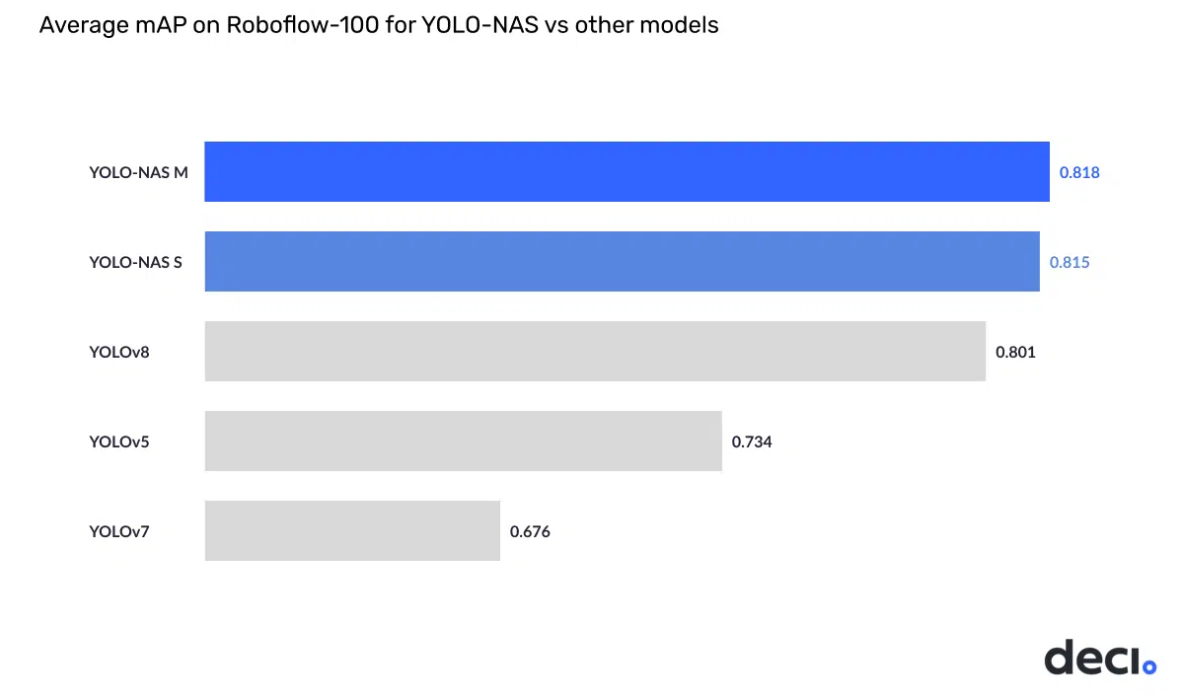
\includegraphics[width=\linewidth]{YOLO-NASSM_vs_other_models.PNG}
    \caption{Average mAP on Roboflow-100 \\for YOLO-NAS vs other models.}
    \label{fig:YOLO-NASSM_vs_other_models}
  \end{minipage}%
  \begin{minipage}{0.5\textwidth}
    \centering
    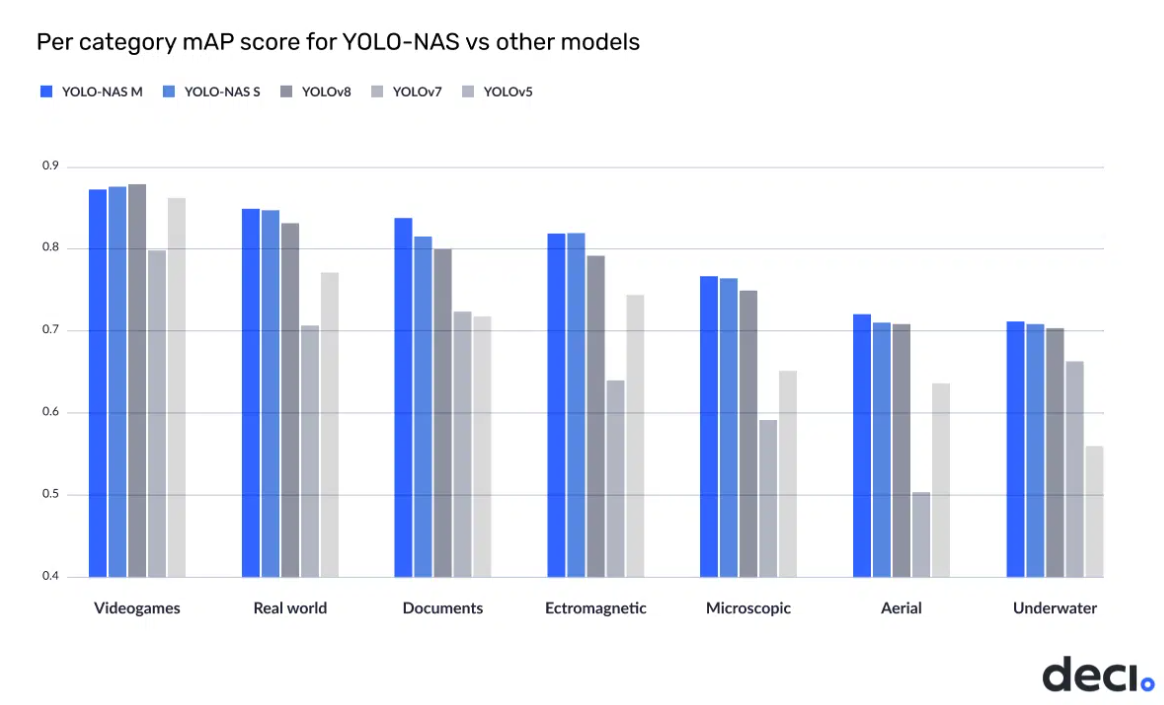
\includegraphics[width=\linewidth]{YOLO-NAS_vs_other_models.PNG}
    \caption{Per category mAP score for YOLO-NAS vs other models.
    Note: For Yolo vV5/v7/v8}
    \label{fig:YOLO-NAS_vs_other_models}
  \end{minipage}
  \caption{Average mAP and Per category mAP score for YOLO-NAS vs other models.}
\end{figure}
Figure \ref{fig:YOLO-NASSM_vs_other_models} are the results obtained by focusing on the “Small” and “Medium” YOLO-NAS variants, and figure: \ref{fig:YOLO-NAS_vs_other_models} is a per-category breakdown of YOLO-NAS’s performance on the RF-100 dataset, compared to the performance of v5/v7/v8 models. \cite{YOLO-NAS}, \cite{yolo-nas-v8-sota}
\href{https://deci.ai/blog/yolo-nas-object-detection-foundation-model/}{\textcolor{blue}{Source}}
\subsubsection{Object Detection Evaluation Metrics}
Object detection metrics are measures used to evaluate the performance of object detection algorithms
Performance metrics are key tools to evaluate the accuracy and efficiency of object detection models. They shed light on how effectively a model can identify and localize objects within images. Additionally, they help in understanding the model's handling of false positives and false negatives. These insights are crucial for evaluating and enhancing the model's performance.
There are many evaluation metrics and the following are broadly applicable accross different object detection, also specifically in YOLO-NAS model. \cite{metrics}
\href{https://docs.ultralytics.com/guides/yolo-performance-metrics/#object-detection-metrics}{\textcolor{blue}{Source}}
\begin{itemize}
    \item \textbf{Intersection over Union (IoU):} IoU is a measure that quantifies the overlap between a predicted bounding box and a ground truth bounding box. It plays a fundamental role in evaluating the accuracy of object localization.
    \item \textbf{Average Precision (AP):} AP computes the area under the precision-recall curve, providing a single value that encapsulates the model's precision and recall performance.
    \item \textbf{Mean Average Precision (mAP):} mAP extends the concept of AP by calculating the average AP values across multiple object classes. This is useful in multi-class object detection scenarios to comprehensively evaluate the model's performance.
    \item \textbf{Precision and Recall:} Precision quantifies the proportion of true positives among all positive predictions, assessing the model's capability to avoid false positives. On the other hand, Recall calculates the proportion of true positives among all actual positives, measuring the model's ability to detect all instances of a class.
    \item F1 Score: The F1 Score is the harmonic mean of precision and recall, providing a balanced assessment of a model's performance while considering both false positives and false negatives.
\end{itemize}

\subsubsection{Benefits of YOLO-NAS over other models}
\textbf{Optimized Efficiency: }\\
YOLO-NAS excels in achieving an optimal balance between accuracy and speed, surpassing other human-designed models in terms of efficiency. This optimization plays a pivotal role in enhancing inference speeds and improving resource utilization, which are essential for the demands of real-time object detection applications.\\
\textbf{Adaptability to Diverse Tasks and Hardware: }\\
YOLO-NAS’s architecture makes it adaptable to a variety of object detection tasks, ranging from common objects to more intricate scenarios and hardware. This versatility positions YOLO-NAS as a valuable tool across a spectrum of applications.\\
\textbf{Training on Prominent Datasets: }\\
YOLO-NAS enhances its capabilities through pre-training on the well established Object365, followed by training on COCO. This strategic pre-training equips the model with a comprehensive understanding of common object features, significantly boosting its accuracy when presented with new and previously unseen images.\\
\textbf{Detection and Localization Accuracy: }\\
YOLO-NAS specialized architecture adeptly addresses challenges associated with small or intricate objects, providing not only heightened detection capabilities but also improved accuracy in pinpointing precise locations. These advancements position YOLO-NAS as a superior choice for a diverse range of applications, especially those where identifying small or elusive objects is pivotal. While YOLOv8 is an impressive object detection model, it encounters limitations when tasked with the intricate challenge of small object detection and localization accuracy. Although proficient in various scenarios, YOLOv8 falls short compared to the specialized capabilities of YOLO-NAS in handling challenges posed by diminutive objects. \cite{yolo-nas-vs-yolov8}
\begin{figure}[H]
    \centering
    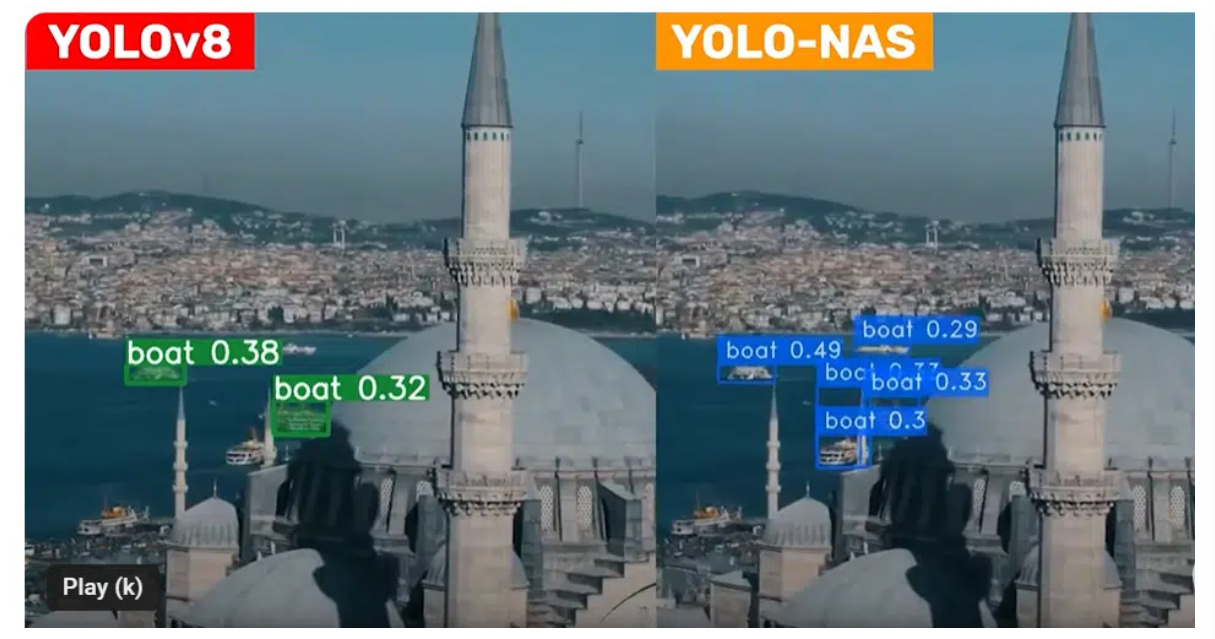
\includegraphics[width=0.7\textwidth]{YOLO-V8_vs_YOLO-NAS.PNG}
    \caption{Performance evaluation on YOLO-V8 vs. YOLO-NAS \href{https://www.youtube.com/watch?v=uPgE8G4CGF4}{\textcolor{blue}{Source}}}
    \label{Yolo-V8_vs_YOLO-NAS}
\end{figure}


\subsubsection{Data set}
\label{datset}
The "p4p Cars Computer Vision Project" stands as a meticulously curated dataset within the Roboflow Universe, purposefully designed for object detection, with a specific emphasis on vehicular recognition. Encompassing a diverse array of vehicle types, including buses, cars, motorbikes, trucks, and vans, this dataset plays a crucial role in advancing computer vision applications.

In terms of key attributes, the project adopts an object detection framework with distinct classes such as bus, car, motorbike, truck, and van. The dataset comprises 10,000 images, with data allocation distributed as 70\texttt{\%} for training, 20\texttt{\%}for validation, and 10\texttt{\%} for testing.

Data preprocessing involves the application of Auto-Orient, resizing images to 640x640 with a stretch mechanism, and modifying classes with 0 remapped and 0 dropped instances. Notably, no augmentations were applied during the preprocessing phase.

This dataset holds substantial utilitarian significance across various domains. It facilitates real-time traffic monitoring and analysis, contributing to the refinement of overarching traffic management strategies. Additionally, it enables security entities to identify and catalog vehicles entering or exiting specific zones. The dataset serves as a valuable reservoir of training data for autonomous driving technologies, aiding self-driving vehicles in discerning between distinct vehicle classes on road networks. Enterprises relying on vehicular fleets, encompassing rental, logistics, or transportation sectors, can leverage the dataset for automatic classification, optimizing inventory management protocols. Moreover, insurance and law enforcement agencies find utility in expediting the analysis of accident scenes, where automatic identification of involved vehicle classes streamlines claims adjudication and investigative procedures.

The "p4p Cars Computer Vision Project" dataset epitomizes substantive potential across domains, ranging from traffic management and security to autonomous vehicles, fleet management, and traffic accident analysis.\cite{p4p-cars_dataset}

